
% Costruzione con i nodi del triangolo di Tartaglia.

\chapter{Tartaglia}
\label{iiChTartaglia}

In questo capitolo utilizzeremo le funzionalità di creazione dei nodi per
realizzare il triangolo di Tartaglia. I nodi sono oggetti tipografici pronti da
posizionare sulla pagina che vengono prodotti da \TeX{} in uno degli ultimi
momenti del processo. \LuaTeX{} è in grado di creare i nodi anche per altra via,
tramite la creazione di oggetti in Lua.

I nodi sono di vario tipo, per esempio dimensioni elastiche o glifi, e vengono
assemblati in liste anche molto complesse perché strutturate in scatole
verticali od orizzontali. Infine, senza entrare troppo nel dettaglio tecnico, i
nodi non rientrano nella gestione automatica della memoria operata dal Garbage
Collector di Lua, mentre occorre programmare correttamente i riferimenti
al nodo seguente e precedente se si vuole creale una lista.

Per questi motivi conviene manipolare le liste dei nodi attraverso le funzioni
che si trovano nella tabella \code{node}, anziché operare su di essi
direttamente.

Con i nodi ogni dettaglio deve essere costruito. Si opera come un tipografo
che lavora con strumenti elementari, assemblando un pezzo alla volta.


\section{Costruzione del triangolo di Tartaglia}

Il Triangolo di Tartaglia%
\footnote{\url{https://it.wikipedia.org/wiki/Triangolo_di_Tartaglia}.} fino
all'ottavo livello è qui rappresentato:
\begin{center}
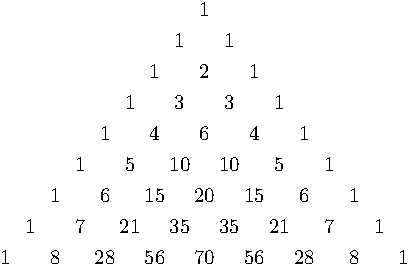
\includegraphics{image/tart-triangolo.pdf}
\end{center}

Ogni nuovo livello è costruito sul precedente sommando i due interi che
sovrastano un dato elemento in modo che il primo e l'ultimo numero siano sempre
1. La proprietà più nota del triangolo è che il livello \( n \) è formato dai
coefficienti binomiali \( (a + b)^n \).

Procediamo con il codice. Chiudete la guida e cercate una vostra implementazione
in \LuaTeX{} stampando i numeri dei livelli fino all'ottavo su una stessa linea
separandoli con uno spazio. Confrontate poi la soluzione fornita nel prossimo
listato.

Al solito stiamo procedendo per gradi. Otteniamo prima il codice che produce i
numeri del triangolo e poi il codice che costruisce la lista dei nodi da
inserire in una scatola che lo compone sulla pagina.

Ecco la mia versione, che utilizza una sola tabella che cresce livello dopo
livello:
\sourcecode{file = [[app-tartaglia/01.tex]]}


\section{Nodi}

I numeri del triangolo vanno posizionati in punti ben precisi. Otterremo
la disposizione geometrica regolando le distanze tra i gruppi di cifre in modo
che il centro del testo che rappresenta un numero sia sull'asse verticale
opportuno per il livello, e disponendo una scatola sull'altra per l'insieme dei
livelli. I passi che svolgeremo in plain \LuaTeX{} sono i seguenti:
\begin{compactenumerate}
\item comporre una cifra,
\item comporre un numero in una lista,
\item comporre più numeri in linea congiungendo le liste con un nodo spazio,
\item assemblare una scatola sull'altra.
\end{compactenumerate}


\subsection{Un numero}

Per costruire un nodo di tipo glifo, un singolo elemento nella collezione
di un font, si utilizza la funzione \fn{node.new}. Poi è obbligatorio
valorizzare almeno il codice del carattere per il campo \code{char} e il numero
del font per il campo \code{font}.

Ottenuto l'oggetto nodo possiamo comporlo sulla pagina con la funzione
\fn{node.write}. Per esempio se volessimo stampare un 8:
\sourcecode{file = [[app-tartaglia/02.tex]]}

La macro \cs{leavevmode} è importante perché è vietato inserire un oggetto glifo
in modo verticale, ed è questa la modalità in cui si trova \TeX{} all'inizio.


\subsection{Dal numero alla lista}

Dal numero, con l'operatore modulo a 10 è possibile ricavare in un ciclo le
cifre componenti la rappresentazione decimale a partire da quella meno
significativa. Con la singola cifra si crea il glifo e lo si concatena in una
lista tramite la funzione \fn{node.insert\_before} che funziona anche per
aggiungere un elemento in testa.

Curando il caso particolare dello zero, questo è quello che fa la funzione
\fn{digit} nel seguente sorgente compilabile:
\sourcecode{file = [[app-tartaglia/03.tex]]}

Il metodo \fn{node.write} accetta un nodo e non una lista. Ma se il nodo
argomento ha un riferimento a un nodo nel campo \code{next}, verrà composta
tutta la catena. Questi riferimenti sono stati inseriti per noi da
\fn{node.insert\_before}.

Dunque la lista costruita è la sequenza di glifi delle cifre del numero 12090.
Dobbiamo ricordarci che il testo composto che ne risulta è tipografia minimale,
perché la lista non è stata modificata per inserire legature, kerning, o punti
di cesura a fin di riga. Con i nodi siamo noi gli artigiani digitali.


\subsection{Numeri e spazi}

Un nodo \emph{glue} distanzia il nodo precedente da quello successivo, in
orizzontale. Può essere elastico in estensione o riduzione, oppure rigido.
Per il nostro scopo dovremo calcolare la distanza rigida tra i nodi in modo
tale che i centri dei due numeri successivi a un livello del triangolo distino
sempre lo stesso valore.

Occorre quindi misurare la larghezza del numero composto. La cosa più semplice è
inserire la lista dei nodi glifo in una scatola orizzontale per poi misurarla
con la funzione \fn{node.dimensions} che ne restituisce larghezza, altezza sulla
lina base e profondità dalla linea base.

La dimensione tra due scatole dovrà essere la differenza tra la distanza assiale
con la semisomma delle larghezze delle scatole adiacenti.

Il passo successivo è quindi aggiungere la funzione \fn{pack\_level} per
costruire la scatola orizzontale contentente la lista di un livello intero del
triangolo di Tartaglia a partire dalla tabella di interi.

Una scatola orizzontale di una lista si costruisce passando il nodo capolista
alla funzione \fn{node.hpack}. nel codice ho modificato la funzione \fn{digits}
affinché restituisca due paramentri: il nodo della scatola orizzontale che
contiene la lista dei nodi glifi e la larghezza della scatola stessa.

Il sorgente compilabile diventa questo:
\sourcecode{file = [[app-tartaglia/04.tex]]}

\begin{figure}
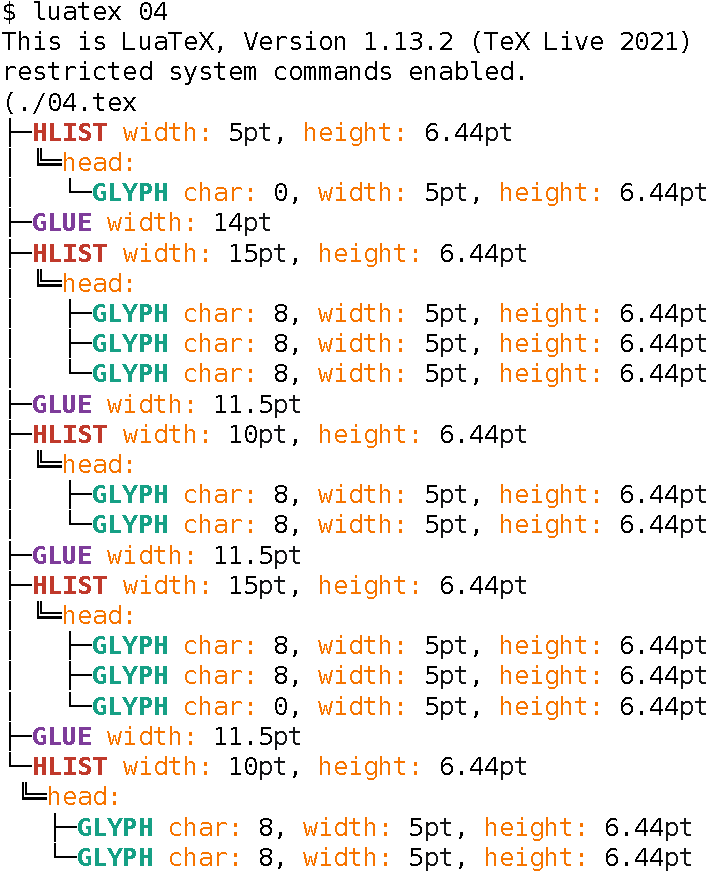
\includegraphics[scale=0.62]{image/nodetree-list-crop.pdf}
\caption{Rappresentazione della lista dei nodi contenuta nella variabile
\code{list} del listato \key{04.tex} modificato per l'utilizzo del pacchetto
\code{nodetree}. Si può notare che i nodi glue tranne il primo hanno lunghezza
di 11,5pt perchè le cifre adiacenti sono sempre di due e tre cifre, il che porta
a calcolare sempre la stessa distanza per mantenere quella assiale di 24pt con
cifre larghe 5pt.}
\label{figNodetree}
\end{figure}

Se esageriamo con la grandezza dei numeri allora si sovrapporrano. Questo
succede se la lunghezza elastica è negativa poiché la distanza assiale di 24pt
(vedi la variabile locale \key{'a'}) è troppo piccola. A questo livello del
codice, l'utente deve controllare che non ci siano sovrapposizioni specie
all'ultima riga del triangolo dove si trovano i numeri più grandi.


\subsection{Intermezzo: debug di una lista di nodi}

Per visualizzare i nodi di una lista per scopi di debug è possibile usare il
pacchetto \pack{nodetree} \cite{pkg:nodetree} di Josef Friedrich. Uno dei modi è
caricare la libreria omonima e usare la funzione
\fn{nodetree.print}\luastd{nodetree.print} per stampare a terminale la
rappresentazione dell'albero contenuta nel nodo passato come argomento:
\begin{lines}
local list = ...
local nodetree = require "nodetree"
nodetree.print(list)
\end{lines}

La documentazione del pacchetto fornisce i dettagli delle opzioni, per esempio
per regolare la quantità d'informazioni tramite il parametro \opz{verbosity} o
per impostare stili di stampa. L'output può essere dirottato verso un file,
specie quando comprende numerose linee di testo.

Con questa tecnica la stampa della rappresentazione dell'albero dei nodi della
lista di numeri spaziati ottenuta alla sezione precedente con il codice del file
\code{04.tex}, e contenuta nella variabile \key{list}, è riportata nella
figura~\ref{figNodetree}.

Con \code{nodetree} si possono incontrare problemi se il terminale non è
compatibile con i codici di colori e con alcuni caratteri grafici usati per
collegare i nodi.


\begin{figure}[b]
\centering
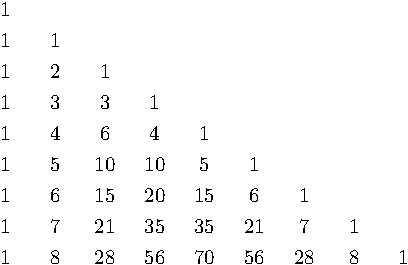
\includegraphics{image/tart-left}
\caption{Triangolo di Tartaglia allineato a sinistra, ottenuto con il listato
\code{05.tex}.}
\label{figTriangoloTartagliaLeft}
\end{figure}

\subsection{Sovrapposizione scatole}

Il passo finale è quello di sovrapporre le scatole orizzontali a formare il
triangolo. Basterà impacchettare le scatole in una scatola verticale con la
funzione \fn{node.vpack} dopo aver costruito la lista di scatole e spazi
verticali.

Dobbiamo prima modificare la funzione \fn{pack\_level} perché restituisca una
scatola orizzontale per il materiale di un intero livello. Fino a ora la lista
poteva anche essere una sequenza di scatole e nodi glue perché la immettevamo in
modo orizzontale. Adesso invece immettiamo le righe del triangolo in ambiente
verticale impacchettando la lista delle righe separate con un nodo di lunghezza
con la funzione \fn{node.vpack}.

Queste sono le nuove funzioni: \fn{next\_level} calcola la riga del triangolo
rispetto a quella precedente, e \fn{tartaglia} genera il triangolo fino al
livello specificato in una scatola verticale:
\begin{lines}
#[indexfile=app-tartaglia/05.tex]
-- filename: app-tartaglia/05.tex
local function next_level(t, row)
    t[row+1] = 1
    for e = row, 2, -1 do
        t[e] = t[e] + t[e-1]
    end
end
local function tartaglia(level)
    assert(type(level)=="number")
    local il = tex.sp "8.5pt"
    local head, last
    local t = {}
    for l = 0, level do
        next_level(t, l)
        local hbox = pack_level(t)
        if head then
            local g = node.new("glue")
            g.width = il
            head, last = node.insert_after(head, last, g)
            head, last = node.insert_after(head, last, hbox)
        else
            head, last = node.insert_after(head, last, hbox)
        end
    end
    local vbox = node.vpack(head)
    return vbox
end
\end{lines}

Il risultato è quello della figura~\ref{figTriangoloTartagliaLeft}.


\subsection{Opzione allineamento}

Per allineare al centro o a destra le linee possiamo introdurre dei nodi
lunghezza nella scatola orizzontale della singola riga. Conviene inserire questi
nodi con la funzione \fn{pack\_level} perché se lo facessimo all'esterno dovremo
poi reimpacchettare la lista in un'ulteriore scatola orizzontale per poterle poi
sovrapporre in ambiente verticale.

A questo scopo aggiungeremo il parametro \code{align}. Per dimostrare quanto si
riveli utile la dinamicità del linguaggio Lua, considereremo tre diversi
possibili gruppi di valori di tipo diverso per il parametro:
\begin{compactitemize}
\item \code{align} vale \key{nil}, per esempio perché nella chiamata di funzione
principale il valore non è stato assegnato: l'allineamento assume il valore di
default di triangolo centrato;
\item \code{align} è una stringa, allora potrà valere \code{"left"},
\code{"center"} o \code{"right"};
\item \code{align} è un numero come frazione di spazio che deve rimanere a
sinistra del primo elemento in alto. Quindi 0 è la stessa cosa dell'allineamento
\code{"left"}, \( 1/2 \) di \code{"center"} e 1 di \code{"right"}. Sono
possibili valori negativi o maggiori di 1.
\end{compactitemize}

Il trucco per implementare facilmente l'aggiunta delle lunghezze di allineamento
davanti e in coda alla lista degli elementi di un livello del triangolo è quello
di conoscere quanto vale lo spazio \( w \) da distribuire opportunamente.

Al livello \( r \), se \( a \) è la distanza assiale tra numeri adiacenti e \(
r_\mathrm{tot} \) è il numero totale dei livelli, allora \( w \) vale:
\[
w = k_\mathrm{left} + k_\mathrm{right} = a\left(r - r_\mathrm{tot}\right)
\]

L'esattezza matematica dell'espressione è dovuta al fatto che il numero in testa
e in coda per ogni riga del triangolo è sempre 1.

Il listato completo della funzione \fn{pack\_level} è il seguente:
\begin{lines}
#[indexfile=app-tartaglia/06.tex]
-- filename: app-tartaglia/06.tex
local function pack_level(t, diff_level, k_left, k_right)
    local a = tex.sp "24pt"
    local w1
    local head, last
    if diff_level == 0 then
        k_left, k_right = nil, nil
    end
    if k_left then
        head = node.new("glue")
        head.width = a*diff_level*k_left
        last = head
    end
    for _, n in ipairs(t) do
        local hbox, w2 = pack_digits(n)
        if w1 then
            local g = node.new("glue")
            g.width = a - (w1+w2)/2
            w1 = w2
            head, last = node.insert_after(head, last, g)
            head, last = node.insert_after(head, last, hbox)
        else
            w1 = w2
            head, last = node.insert_after(head, last, hbox)
        end
    end
    if k_right then
        local g = node.new("glue")
        g.width = a*diff_level*k_right
        head, last = node.insert_after(head, last, g)
    end
    return node.hpack(head)
end
\end{lines}

La funzione tiene conto delle situazioni in cui non è necessario inserire il
distanziamento di allineamento su un lato, cioè quando la lunghezza vale zero
oppure quando la linea da impacchettare è l'ultima, riga che non ha mai
necessità di essere traslata.

Tuttavia, non viene fatto affidamento sulla \emph{direzione di composizione} per
allineare a destra o a sinistra e viene inserito sempre lo spazio. Se
l'allineamento fosse a sinistra le scatole sarebbero allineate a sinistra dal
compositore che dispone gli oggetti in modo orizzontale da sinistra a destra. Ma
se la direzione fosse impostata al contrario l'effetto sarebbe l'opposto.

Per questo nel codice viene inserita la lunghezza a destra nonostante
l'allineamento a sinistra. I parametri \( k_\mathrm{left} \) e \(
k_\mathrm{right} \) sono definiti dalla funzione principale \fn{tartaglia} a
seconda del parametro \code{align}. Il listato è il seguente:
\begin{lines}
#[indexfile=app-tartaglia/06.tex]
-- filename: app-tartaglia/06.tex
local function tartaglia(level, align)
    assert(type(level)=="number")
    local k_left, k_right; if align then
        if type(align) == "string" then
            if align == "center" then
                k_left, k_right = 0.5, 0.5
            elseif align == "right" then
                k_right = 1
            elseif align == "left" then
                k_left = 1
            end
        elseif type(align) == "number" then
            if align == 0 then
                k_right = 1
            elseif align == 1 then
                k_left = 1
            else
                k_left, k_right = align, 1 - align
            end
        else
            error("Unexpected alignment value")
        end
    else
        k_left, k_right = 0.5, 0.5
    end
    local il = tex.sp "8.5pt"
    local head, last
    local t = {}
    for l = 0, level do
        next_level(t, l)
        local hbox = pack_level(t, level - l, k_left, k_right)
        if head then
            local g = node.new("glue")
            g.width = il
            head, last = node.insert_after(head, last, g)
            head, last = node.insert_after(head, last, hbox)
        else
            head, last = node.insert_after(head, last, hbox)
        end
    end
    local vbox = node.vpack(head)
    return vbox
end
\end{lines}

Domanda: se avessimo avuto numeri diversi da 1 come primo e ultimo elemento, se
ritenuto necessario, quali modifiche occorrebbe considerare nel codice?


\subsection{Verifica grafica degli allineamenti con TikZ}

Per controllare visivamente gli allineamenti verticali nel triangolo di
Tartaglia è possibile sovrapporre linee verticali sottili di passo \( a \) al
disegno. Realizzare questo disegno è in realtà molto semplice poiché una volto
costruito il nodo del contenitore, la scatola può essere assegnata direttamente
a uno dei registri tramite indicizzazione della tabella \code{tex.box}:
\begin{lines}
#[tex]
% !TeX program = LuaTeX
\newbox\tartbox % nuovo registro
\directlua{
    ... definizioni come prima
    tex.box.tartbox = tartaglia(8)
}
\box\tartbox
\bye
\end{lines}

La macro \cs{box} è una primitiva di \TeX{}. Quello che fa è comporre sulla
pagina il contenuto del box indicato dalla control sequence che lo segue e poi
svuotarlo.

A questo punto è facile separare la costruzione del triangolo dal suo impiego, e
un esempio è proprio far espandere la scatola in una macro \cs{node} del
pacchetto grafico TikZ:
\begin{lines}
#[tex]
#[indexfile=app-tartaglia/07.tex]
% !TeX program = LuaTeX
% filename: app-tartaglia/07.tex
\input tikz.tex
\newbox\tartbox
% ...
\directlua{
    ... definizioni come prima
    tex.box.tartbox = tartaglia(8)
}
\tikzpicture
\foreach \x in {-96,-72,...,96} {
\draw[blue] (\x pt,68pt) -- (\x pt,-68pt);
}
\foreach \x in {-84,-60,...,84} {
\draw[red] (\x pt,68pt) -- (\x pt,-68pt);
}
\node at (0, 0) {\box\tartbox};
\endtikzpicture
\bye
\end{lines}

Le rette rosse e quelle blue distano 24pt una dall'altra. Sono posizionate a
partire dall'ascissa zero poiché TikZ inserirà la scatola usando il suo punto
centrale nell'origine del sistema di riferimento.

Le linee rosse corrispondono alle posizioni dei numeri sui livelli dispari,
e quelle blu a quelle dei livelli pari. Il risultato è:
\begin{center}
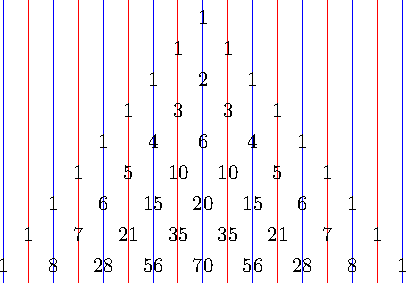
\includegraphics{image/tart-tikz.pdf}
\end{center}


\subsection{Regolazione automatica della distanza}

Sappiamo che la distanza \( a \) tra i centri di due numeri consecutivi su una
linea del triangolo è fissa. Se non fosse abbastanza grande i due numeri si
sovrapporrebbero e a quel punto l'utente dovrebbe reimpostarne il valore nel
sorgente e ricompilare.

Possiamo invece rendere l'operazione automatica e in diversi modi. Per esempio,
potremo intendere che il triangolo venga costruito in base a una distanza minima
tra un numero e l'altro, oppure impostando la distanza \( a \) come fissa per
incrementarla in caso di sovrapposizioni.

Una prima soluzione è costruire la scatola con il triangolo solo alla fine,
salvare cioè le scatole orizzontali dei numeri in una tabella e nel frattempo
calcolarne il valore minimo di \( a \); costruire poi la scatola contenitore del
triangolo distanziando opportunamente i nodi.

Una seconda strada è quella di impacchettare il triangolo come fatto fino a ora
negli esempi, per poi eventualmente scorrere la lista dei nodi per incrementare
la distanza tra i centri. Questa seconda strategia è quella che seguirò per
mostrare come una lista di nodi già costruita possa essere utilmente
modificata.


% \subsection{Visitare la lista dei nodi}

% missing material

\subsection{Modificare la distanza}

Useremo la funzione \fn{pack\_level} per creare la lista di un livello del
triangolo di Tartaglia già scritta in precedenza, e una nuova funzione
\fn{add\_distance} per modificare la distanza tra i centri.

Alcune informazioni utili tratte dal manuale di \LuaTeX{} che è bene richiamare:
la lista contenuta in un nodo scatola orizzontale o verticale inizia con il nodo
contenuto nel campo \code{head}. Nella lista il nodo successivo può essere
ricavato leggendo il campo \code{next} del nodo attuale. Il campo numerico
\code{id} indica il tipo di nodo, per esempio 12 individua un nodo \code{glue} e
0 un nodo \code{hbox}.

Aggiungere una distanza fissa è molto semplice. Sappiamo che il nodo \code{hbox}
è l'alternanza tra scatole orizzontali e nodi \code{glue}, perciò se \code{hbox}
è il mnome di variabile che contiene la scatola, il riferimento
\code{hbox.head.next} punta al primo nodo distanza. In un ciclo \key{while}
scorrere i soli nodi \code{glue} significa saltare un nodo e quindi preparare il
prossimo riferimento con il campo \code{glue.next.next}:
\begin{lines}
#[indexfile=app-tartaglia/08.tex]
-- filename app-tartaglia/08.tex
local function add_distance(hbox, d)
    assert(hbox and hbox.id == 0)
    local glue = hbox.head.next
    while glue do
        assert(glue.id == 12)
        glue.width = glue.width + d
        glue = glue.next.next
    end
end
\end{lines}

Nel triangolo dobbiamo tener in conto tuttavia degli eventuali nodi di
spaziatura iniziale e finale per l'allineamento orizzontale del triangolo. In
questi spazi l'incremento della distanza è proporzionale alla differenza tra il
numero dei livelli totali con il numero di quello corrente. Dovremo adattare la
funzione \fn{add\_distance} per modificare le lunghezze non solo dei nodi
intermedi tra un numero e l'altro, ma anche per gli eventuali spazi di
allineamento citati, in questo modo:
\begin{lines}
#[indexfile=app-tartaglia/09.tex]
-- filename app-tartaglia/09.tex
local
function add_distance(hbox, d, k_left, k_right, level, totlevel)
    assert(hbox and hbox.id == 0)
    local glue = hbox.head
    local tdist = d*(totlevel - level)
    if k_left then
        assert(glue.id == 12)
        glue.width = glue.width + tdist*k_left
        glue = glue.next
    end
    glue = glue.next
    for _= 1, level do
        assert(glue.id == 12)
        glue.width = glue.width + d
        glue = glue.next.next
    end
    if k_right then
        assert(glue.id == 12)
        glue.width = glue.width +  tdist*k_right
    end
end
\end{lines}

Non si utilizza il ciclo \code{while} ma un ciclo \code{for} che itera tante
volte quanti sono gli spazi nel livello, ovvero il numero del livello a
cominciare da 1 perché il livello 0 non ha spazi intermedi. In questo modo è più
semplice per il codice gestire il puntatore al nodo invece che passare da un
nodo al successivo.

La versione finale contenuta nel file \code{app-tartaglia/09.tex}, conta 160
linee di codice Lua in grado di generare il triangolo di Tartaglia con il numero
di livelli richiesti, diverse opzioni di allineamento orizzontale, e con la
capacità di mantenere la distanza assiale tra i numeri di 24pt più l'eventuale
distanza perché ci siano almeno 3pt tra due numeri consecutivi.

Domanda: se e come cambiereste il codice per considerare la simmetria dei numeri
sulla riga di uno stesso livello del triangolo di Tartaglia?


\section{Riepilogo}

La tecnologia dei nodi consente di comporre oggetti tipografici di complessità
arbitraria. Seguendo vari passi di sviluppo, in questo capitolo abbiamo
costruito con essa il triangolo di Tartaglia, un esempio applicativo
interessante proprio per poter implementare nuove funzionalità come quella di
rendere variabile l'allineamento o lasciare che sia il codice ad aggiustare la
distanza tra i numeri se necessario.

Rimane da esplorare la gestione in Lua delle opzioni e dei parametri perché
l'utente possa modificare l'aspetto del triangolo. Considero questo tema
separato da quello dei nodi di \LuaTeX{}. Per questo motivo l'esercitazione
può dirsi conclusa.


% end of file
